

% Lightbug
\chapter{Lightbug: A (mostly) thought experiment}
\label{chap_lightbug}

   \begin{figure}[thpb]
      \centering
      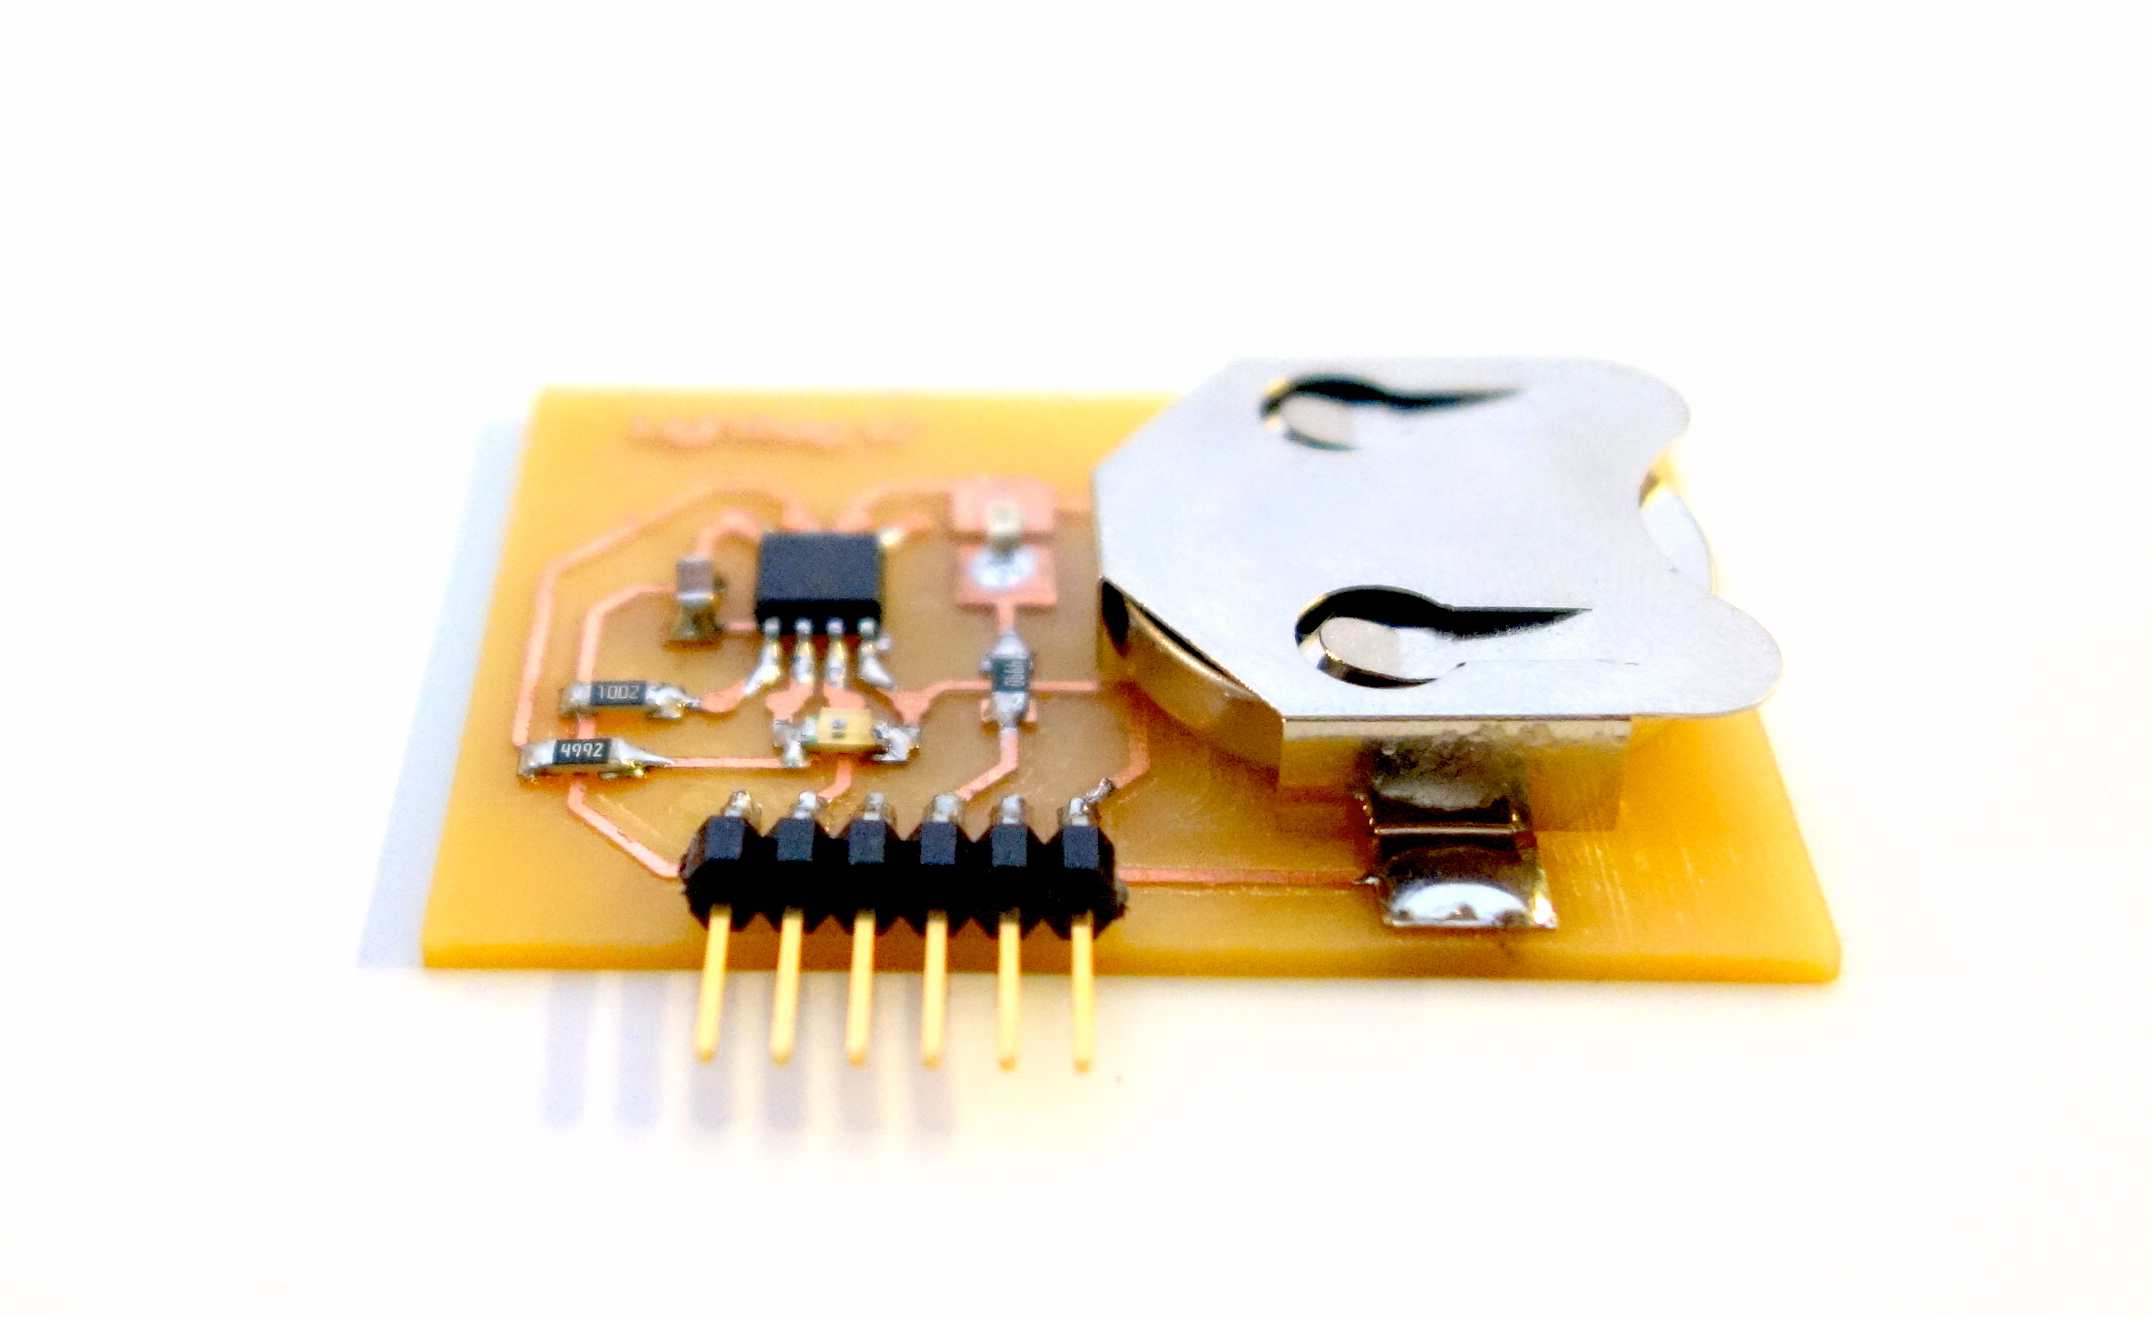
\includegraphics[width=5in]{figures/lightbug/lightbug.jpg}
      \caption{Lightbug v2}
      \label{fig_lightbug}
   \end{figure}



I built a minimal \lq robot\rq , Lightbug, to experience the world and relate its experience. Inspired by Braitenberg's Vehicles \cite{braitenberg_vehicles}, I used a small set of components to isolate the effect of implicit life-story. The Lightbug consists of a light sensor and an LED connected together by a microcontroller and powered by a coin cell battery. The microcontroller, an Atmel AtTiny 45V, provides memory and processing. The Lightbug samples the changing levels of light at intervals and then blinks out what it had seen in a 24 hour period by blinking the LED. The LED is set to high or low brightness depending on how the sampled light compares to a threshold. The threshold is constantly adjusted by an exponential moving average over all the samples of light. A coincell battery, CR2016, can power the Lightbug for few months.  

The experience of seeing a LightBug blinking is being able to get a glimpse of what had happened to it over course of a day interpreted by its own history. I had a few of these scattered throughout my apartment for six months. As variance in lighting was differnet in different location, each differed in the story they created. Over time, I noticed that I was interested in and engaged by the perceived story of the Lightbugs' daily experience some of which was shared by me. At the end of six months, when I had to move, I felt a strong reluctance to turn off the Lightbugs or to put them into storage. 

This personal experiment provided preliminary support for the hypothesis that even minimal ability to experience the world and communicate that experience creates emotional engagement.\marginpar{

      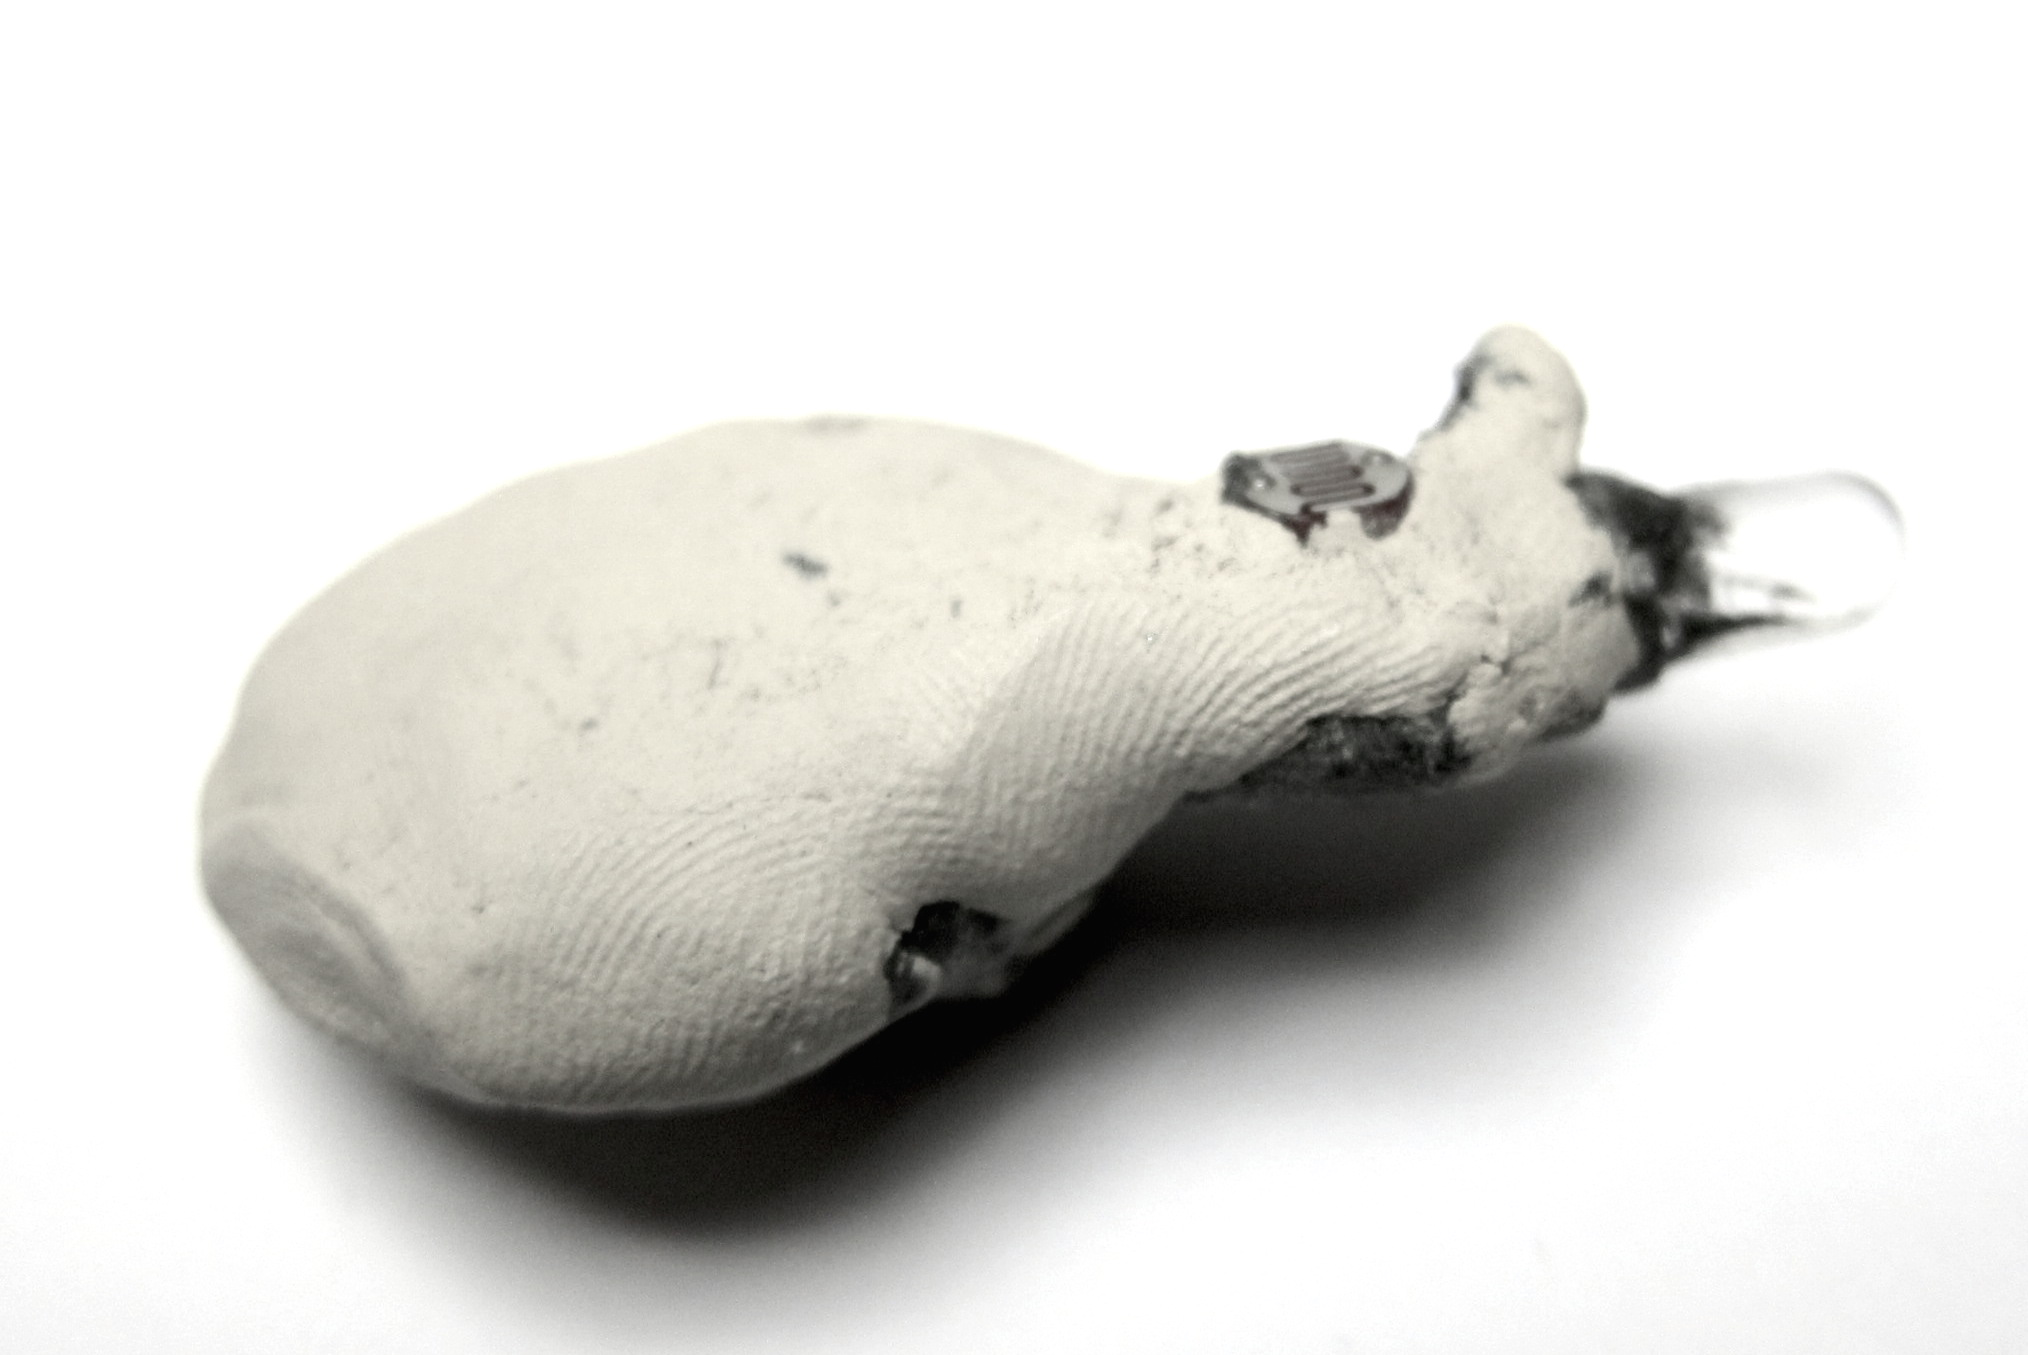
\includegraphics[width=\marginparwidth]{figures/lightbug/lightbug_white.jpeg}
      Early version of Lightbug sealed in epoxy putty.
      %\caption{Juvenile owl used as an inspiration for the sound robot's form design.}

} I found that change was important. There were two kinds of changes that took place: A superficial one which was simply the recording of how bright and dark the light was. Then there was the change in the exponentially decayed threshold which changed how the Lightbug interpreted the brightness. This interpretation made the relating of the experience ambiguous and created room to construct an internal view of the experience.

However, with one subject with vested interest and an active imagination, the study lacked rigor to put it mildly. Moreover, in this experiment, experience was shared by me and I wanted to isolate the effect of just the robot having an experience. 

I constructed a follow-up study in a controlled environment to test the thesis which I will describe in the next chapter. 


% -- joscha

% true love: trascendental purpose. hook that evolution builds into our mind to create society. people are looking for causes to die for. a pointer to something beyond.

% time is probably a big factor. i wouldn't want to spend all this time again. discounted future experience.

% it will go back to being drab.

% it needs to have a goal that it finds meaningful that you are thwarting.

